%%%%%%%%%%%%%%%%%%%%%%%%%%%%%%%%%%%%%%%%%%%%%%%%%%%%%%%%%%
\section{Overview of the Proposed Approach}
\label{sect:overviewApproach}
%%%%%%%%%%%%%%%%%%%%%%%%%%%%%%%%%%%%%%%%%%%%%%%%%%%%%%%%%%

This section explains our basic idea of incorporating behavior aspects as part of a unified domain model.

\begin{figure}[ht]
	\begin{center}
		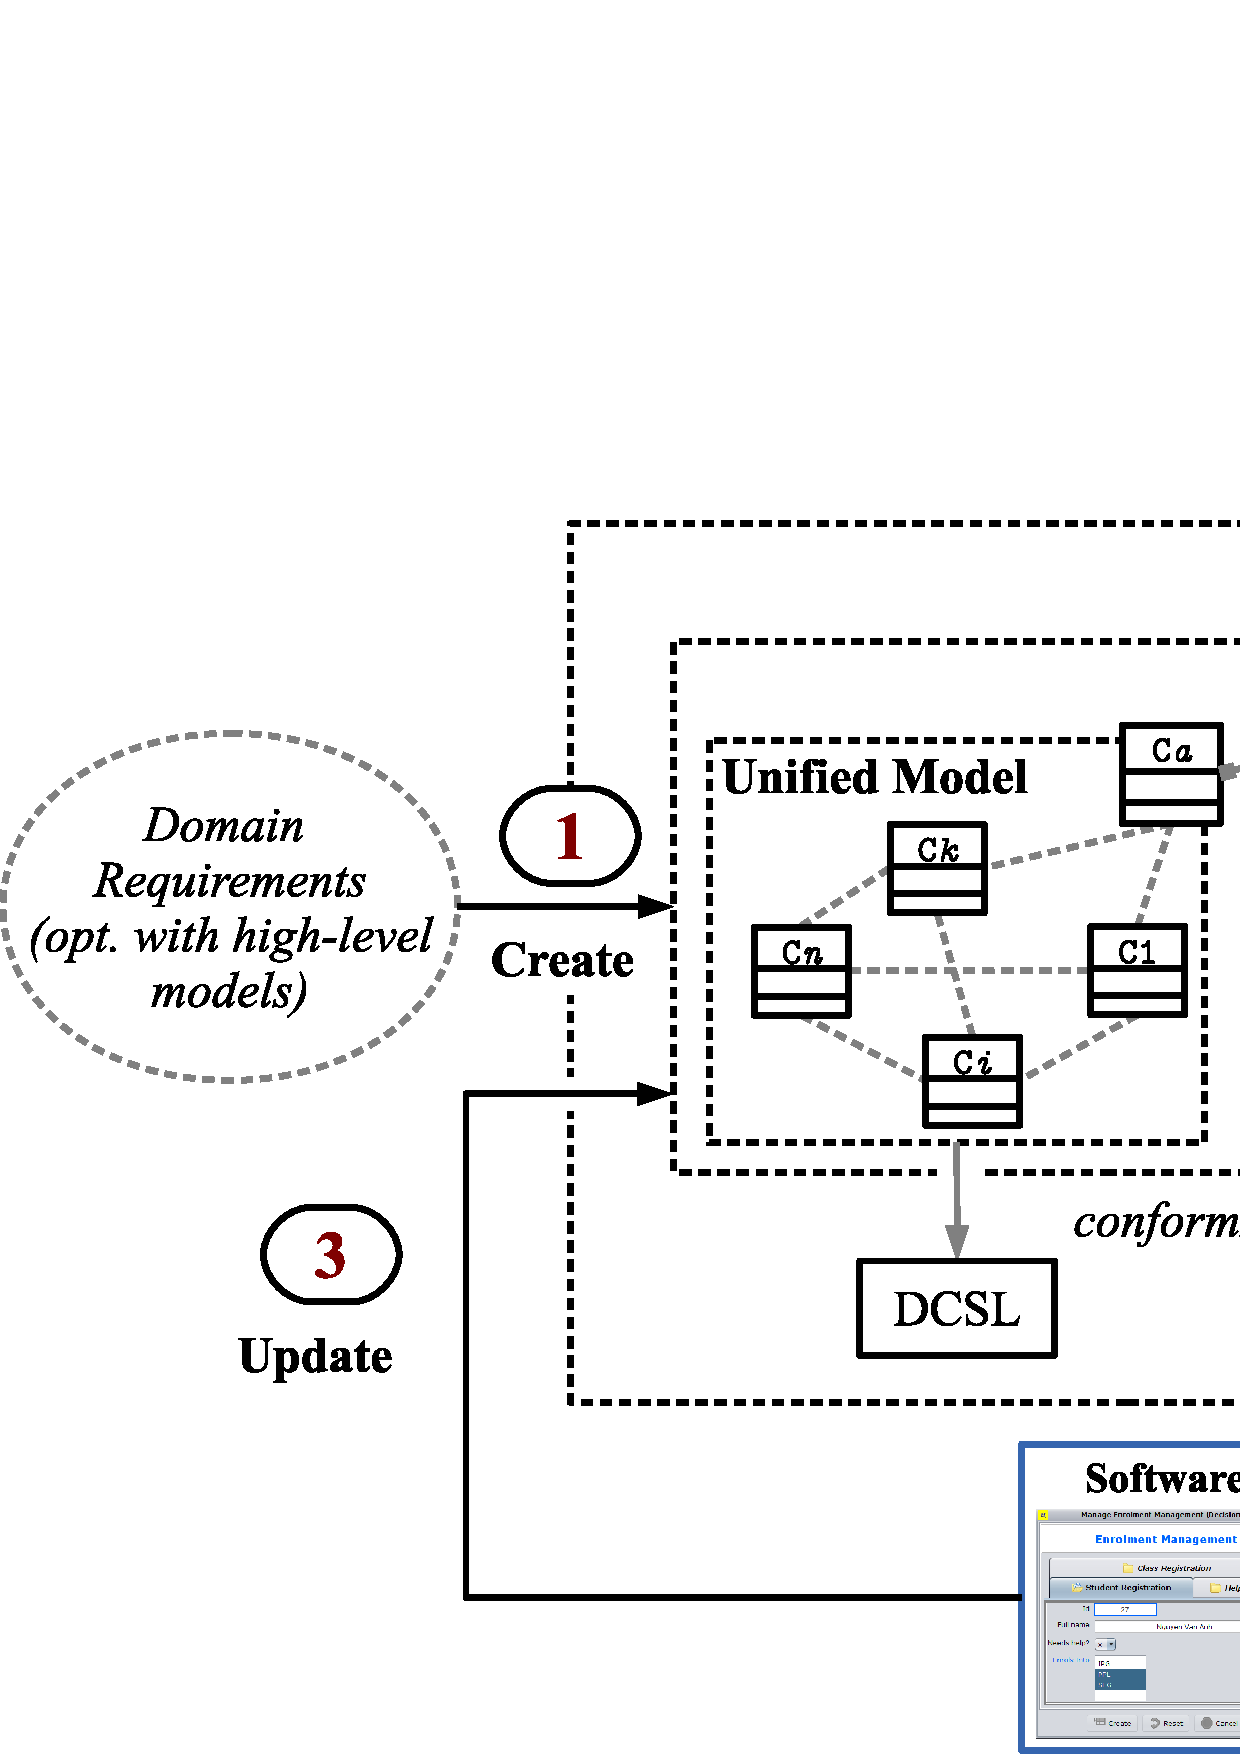
\includegraphics[scale=0.32 %0.26
		]{method-overview}
	\end{center}
	\caption{An overview of our method.} %
	\label{fig:method-overview}
\end{figure}

%%%%%%%%%%%%%%%%%%%%%%%%%%%%%%%%%%%%%%%%%%%%%%
\subsection{Basic Idea}
%%%%%%%%%%%%%%%%%%%%%%%%%%%%%%%%%%%%%%%%%%%%%%

Figure~\ref{fig:method-overview} overviews our proposed method. This method conceptually consists in iteratively performing three steps. First, we take as input domain requirements that are captured by an essential domain model (for a structural view including domain concepts and relationships) together with domain behaviors (specified as a behavioral view with UML Activity diagrams). We then aim to represent such input domain requirements as a composition of a DCSL model for a so-called \textit{unified model} and an \agl~model to represent domain behaviors. The former model (the DCSL model) is an extension of the essential model to relate this structure view with the behavior view. A detailed definition of the unified model is provided in Section~\ref{subsect:unifiedModel}. For the latter model (the \agl~model), wee need to define \agl~as a new aDSL to capture a semantics domain of module actions for the domain behaviors. %
%This semantics domain would be more specific and narrower then the one of UML Activity diagrams. 
A detailed explanation of this point is provided in Section~\ref{subsect:domainBehaviors} and Section~\ref{sect:actSemantics}. %
%
%The figure highlights a unified model and its combination with an activity graph. Here, we consider the unified model as an extended domain model in MOSA~\cite{le_domain_2018}. This model, which is expressed in \dcsl, extends the conventional DDD's domain model~\cite{evans_domain-driven_2004} with the domain-specific features of UML activity diagram. Among the essential features that are supported, an activity class (\eg class \clazz{C_a} in Figure~\ref{fig:method-overview}) is defined for each unified model to represent an activity. We use the activity class as a pivot with which to define the activity graph. Each activity class is attached to an activity graph that describes the behavioral logic of the represented activity. The activity graphs are expressed in the language \agl,~which is explained in Section~\ref{sect:agl}.
%
%Hence, conceptually our method consists in iteratively performing three steps. The first step takes as input the domain requirements, optionally expressed in some high-level models (e.g., UML class and activity diagrams), and creates a set of initial unified models and associated activity graphs. At this stage, the models and their graphs may be incomplete and, thus, need to be refined in subsequent iterations. The second step takes as input the unified models and graphs and uses MOSA to automatically generate a GUI- and module-based software. This software is presented to the domain expert in order to get feedback. If there is feedback, then the third step updates the unified models and graphs and the cycle continues. If, on the other hand, the domain expert is satisfied with the models and graphs, then the cycle ends.
%
Second, the unified model composed with the \agl~model is taken as input to automatically generate a GUI- and module-based software. This software is presented to the domain expert in order to get feedback. %
%
Third, if there is feedback, then the input model will be updated and the cycle continues. If, on the other hand, the domain expert is satisfied with the models, then the cycle ends.

%%%%%%%%%%%%%%%%%%%%%%%%%%%%%%%%%%%%%%%%%%%%%%%%%%%%%%%%%%%%
\subsection{Incorporating Domain Behaviors} 
\label{subsect:domainBehaviors}
%%%%%%%%%%%%%%%%%%%%%%%%%%%%%%%%%%%%%%%%%%%%%%%%%%%%%%%%%%%%

We introduce a mechanism to incorporate domain behaviors into a domain model. The mechanism is defined based on the structure and behavioral semantics of MOSA at two points. %
%
First, each module class that owns a corresponding domain class  is defined with a set of essential actions (i.e., \textit{atomic actions} as explained in Section~\ref{sect:actSemantics}) in order to manipulate the instances of the domain class. %
%We consider these actions as forming a module interface, which is represented by a UML interface named \clazz{ModuleService}. 
%
Second, domain behaviors are considered as collaborations among modules in MOSA: Each module collaboration is on the one hand coordinated by a composite module (in MOSA), on the other hand, captured by a corresponding activity model. Specifically, we map each of the activity models, e.g., the enrolment management in \courseman as depicted in Figure~\ref{fig:motivatingExample2}, to a new domain class (referred to as a so-called activity class that is owned by a corresponding activity module, e.g., the \clazz{ModuleEnrolmentMgmt} in \courseman). The containment tree of the composite module allows promoting it as the main module for managing the entire activity.

%- (Module Interaction Patterns)
Within the proposed mechanism, basically, we could employ UML Activity diagrams to represent domain behaviors but we need to restrict them for a semantics domain corresponding to the behavior semantics of the composite module (coordinating a collaboration among moudules). To define such a semantics domain we employ a pattern-based approach: Domain behaviors are specified using UML Activity diagram with basic constructs corresponding to the five essential activity modeling patterns as presented in~\cite{le_domain_2018}. We named the patterns after these five elementary activity flows: \textit{sequential}, \textit{decisional}, \textit{forked}, \textit{joined} and \textit{merged}. Further explanation for this point is provided in Section~\ref{sect:behaviorPatterns}.
%This paper extends each pattern solution with a specification of the activity graph in the \agl~that is explained in Section~\ref{sect:agl}. 

%%%%%%%%%%%%%%%%%%%%%%%%%%%%%%%%%%%%%%%%%%%%%%%%%%%%%%%%%%
\subsection{Unified Model}
\label{subsect:unifiedModel}
%%%%%%%%%%%%%%%%%%%%%%%%%%%%%%%%%%%%%%%%%%%%%%%%%%%%%%%%%%

A \textit{unified class model} is an extended domain model for incorporating domain behaviors. As explained above, the domain behaviors within our approach are captured as activity models with UML Activity diagrams. Within the extension we newly add so-called \textit{activity classes}, e.g., class \clazz{C_a} in Figure~\ref{fig:method-overview}, for each activity of the domain behaviors. The activity class is referred to and handled by a corresponding activity model (that can be seen as an activity graph) so that the behavioral logic of the activity is realized and synchronized with current states of the domain model. Such a unified class model could be realized in \dcsl~and we refer to the resulting \dcsl~model as a \textit{unified model}.

\begin{definition} \label{def:unified-class-model}
	Let an activity model be specified using a UML activity diagram for domain behaviors. A \textbf{unified class model} \wrt the activity model is a domain model extended with the following features:
	
	\begin{itemize}%[leftmargin=*]
		\item \textbf{activity class}: a domain class that represents the activity.
		\item \textbf{data component class} (or \textbf{data class} for short): a domain class that represents each data store.
		\item \textbf{control component class} (or \textbf{control class}): captures the domain-specific state of a control node. A control class that represents (does not represent) a control node is named after (the negation of) the node type; \eg, decision (non-decision) class, join (non-join) class, \etc
		\item \textbf{activity-specific association}: an association between each of the following class pairs:
		\begin{itemize}
			\item activity class and a merge class.
			\item activity class and a fork class.
			\item a merge (fork) class and a data class that represents the data store of an action node connected to the merge (fork) node.
			\item activity class and a data class that does not represent the data store of an action node connected to either a merge or fork node.
		\end{itemize}        	
	\end{itemize}
	%
	We will collectively refer to the data and control classes of an activity class model as \textbf{component classes}. \qed
\end{definition}

Note that the representation scheme in the above definition does not cover \textit{all} the possible associations among the component classes. It focuses only on the activity-specific ones, i.e., in general, we just focus on a restricted semantic domain of UML Activity diagrams that corresponds to the semantics domain of \agl. % 
%Other domain-specific associations may be introduced if needed.
%
These associations play two important roles. First, they explicitly model the links between domain-specific states of the activity nodes. Second, they are used to incorporate the modules of the data and control classes into the containment tree of the activity module, thereby promoting this module as the main module for managing the entire activity.

The condition imposed on the fourth class pair of activity-specific association stems from the fact that there is no need to explicitly define the association between an activity class and a data class that represents the data store of an action node connected to either a merge or fork node. Such a data class is `indirectly' associated to the activity class, via two associations: one is between it and the merge or fork class (the third class pair), and the other is between the activity class and this control class (the first or second class pair).

%\subsection{Activity Domain Model}
\begin{definition} \label{def:unified-model}
	A \textbf{unified model} is a \dcsl~model that realizes an unified class model as follows:
	\begin{itemize}%[leftmargin=*]
		\item a domain class $ c_a $ (called the \textbf{activity domain class}) to realize the activity class.
		\item the domain classes $ c_1,\dots,c_n $ to realise the component classes.
		\item let $ c_{i_1},\dots,c_{i_k} \in \{c_1,\dots,c_n\} $ realize the non-decision and non-join component classes, then $ c_a,c_{i_1},\dots,c_{i_k} $ contain associative fields that realize the corresponding association ends of the relevant activity-specific associations. \qed
	\end{itemize}
\end{definition}

In the remainder of this paper, to ease notation we will use \textbf{activity class} to refer to the activity domain class $ c_a $ and \textbf{component class} to refer to the $ c_1,\dots,c_n $. 
%We will further assume the existence of a boolean function named \func{activityClass}{:} \clazz{Class} $\rightarrow$ \clazz{Boolean}, which returns \code{true} or \code{false} depending on whether or not a domain class is an activity class.

\begin{figure*}[]
	\begin{center}
		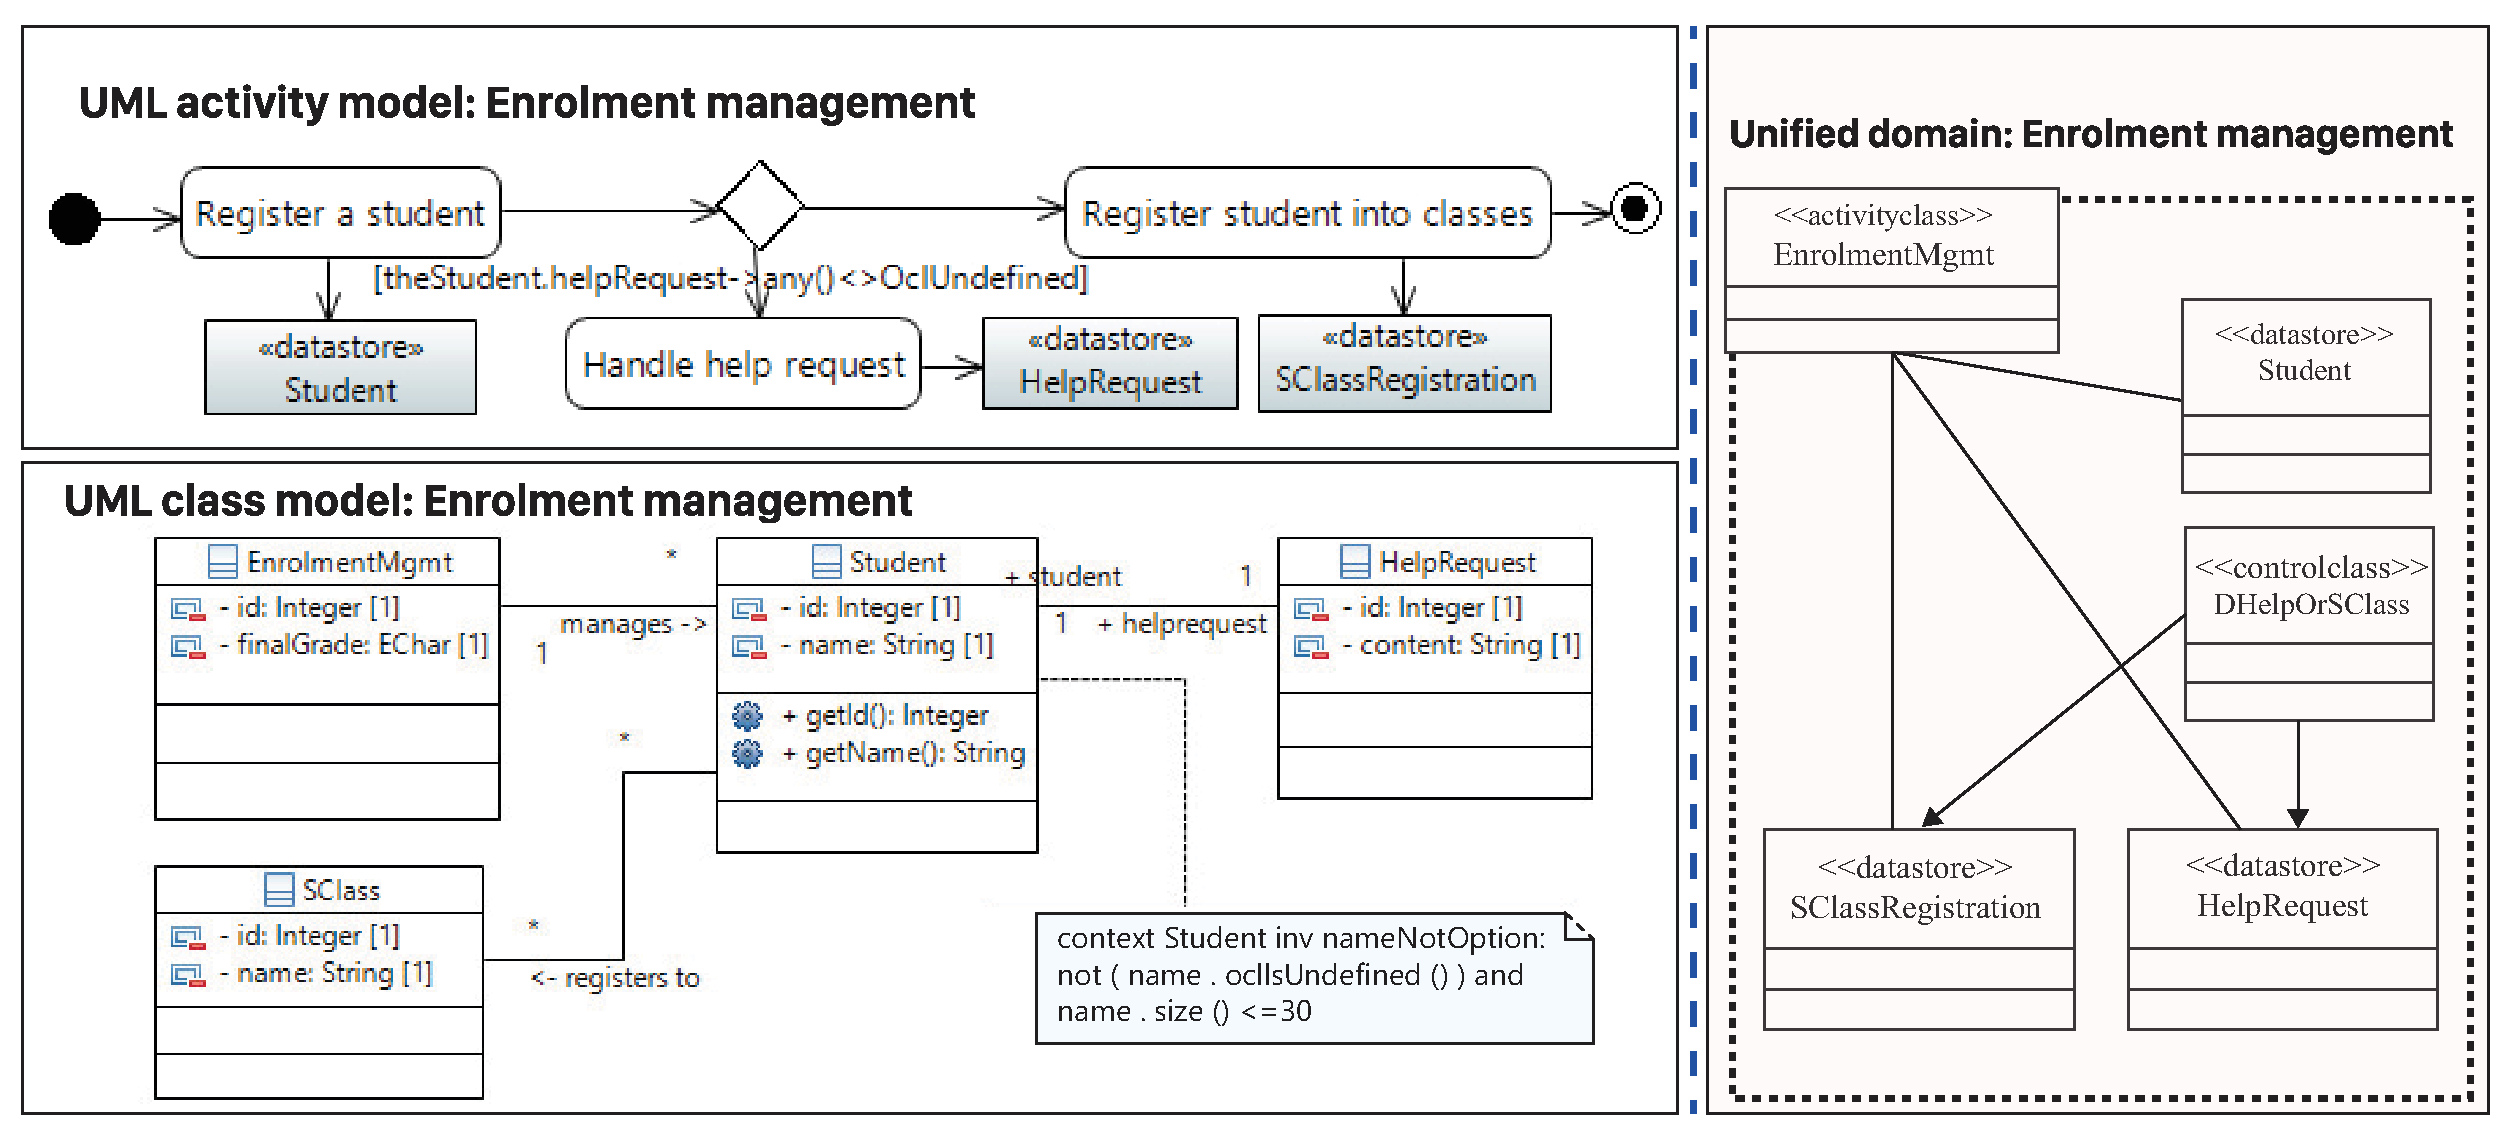
\includegraphics[scale=0.35]{unified-model-example}
	\end{center}
	\caption{(A: Left) The UML activity and class models of a \courseman~software variant that handles the enrollment management activity; (B: Right) The unified model that results.} %
	\label{fig:unified-model-example}
\end{figure*} 

%%%%%%%%%%%
\subsection*{Example: Unified model}
%%%%%%%%%%%

To illustrate, Figure~\ref{fig:unified-model-example}(A) shows the UML activity and class models of a \courseman~variant that handles the enrollment management activity. In this variant, students are allowed to request help after the initial registration. The accompanied class model is extracted from the \courseman's conceptual model as shown in Figure~\ref{fig:motivatingExample}.
%
Figure~\ref{fig:unified-model-example}(B) shows the resulting unified model of the activity.
This model consists of five domain classes and realizations of five activity-specific associations. To ease reading, we omit the domain-specific associations that are shown in the UML class model in Figure~\ref{fig:unified-model-example}(A). Class \clazz{EnrolmentMgmt} is the activity class. Class \clazz{DHelpOrSClass} is a decision class, which captures the domain-specific decision logic. The remaining three classes are data classes that realize the three data stores. These data classes also correspond to three domain classes in the UML class model. 

Among the five associations, three associate \clazz{EnrolmentMgmt} and the data classes. These associations are used to bind the modules of these data classes to the containment tree of \clazz{ModuleEnrolmentMgmt}.
The remaining two associations associate the decision class \clazz{DHelpOrSClass} to two data classes (\clazz{SClassRegistration} and \clazz{HelpRequest}), which realize the data stores connected to the two action nodes branching of the decision node. These associations are weak dependency associations and only added in this case because the decision logic encapsulated by \clazz{DHelpOrSClass} needs to reference the two data classes.
%
%In Section~\ref{sect:behaviorPatterns}, we will revisit this example in the context of the decisional modeling pattern and present a software GUI that is generated from the model.